%!TEX root = ..\main.tex
\section{Model}
\label{sec:model}

\begin{figure*}[t]
\centering
	\includegraphics[width=0.9\textwidth]{Images/fullSystemPicture}
	\caption{Snapshot obtained from Langevin dynamics simulations for density $\rho = 0.95$ and $k_BT = 1.5$. The arrows represent the dipole moment of the particle. The simulation was allowed to equilibrate for Brownian time $t = 33$.}
	\label{fig:fullSystemPicture}
\end{figure*}

We consider colloidal particles with a permanent dipole moment $\mu \hat{m}$, where $\hat{m}$ is a unit vector along the direction of the dipole moment. While considering a three-dimensional system, we constrain particle translational motion to a one-dimensional line, i.e. particles are confined to the $z$ axis. However, particles can explore the full three-dimensional orientation space. A snapshot of the system is shown in the \figref{fig:fullSystemPicture}.

The particle-particle interaction is described as the superposition of two pairwise contributions: a dipole-dipole interaction and a short-range repulsion.

The energy of dipole-dipole pairwise interaction between particles $i$ and $j$ is
\begin{equation}
\label{eq:dipole_dipole_interaction}
U^\mathrm{dip}_{ij} =
	- \frac{\mu_i \mu_j}{\Delta r^3}[
		3 (\hat{m}_i \cdot \hat{r}_{ij})(\hat{m}_j \cdot \hat{r}_{ij})
		- (\hat{m}_i \cdot \hat{m}_j)
	]
\end{equation}
where $\mu_i \hat{m}_i$ and $\mu_j \hat{m}_j$ are the dipole moments of the interacting particles, $\hat{r}_{ij}$ is the unit vector connecting the center of both particles, and $\Delta r$ is the it is the distance between the two particles.

Since the position of the particles is constrained to a line along the z axis, $\hat{r}_{ij}$ is always along with $z$ axis. Assuming that all particles have the same dipole moment $\mu_i = \mu_j \equiv \mu$, and defining $\mu = 1$, Eq. \eqref{eq:dipole_dipole_interaction} can be simplified as,
\begin{equation}
\label{eq:dipole_dipole_1D}
U_{ij}^\mathrm{dip} = - \frac{1}{\Delta z^3} [3 \cos \theta_i \cos \theta_j - (\hat{m}_i \cdot \hat{m}_j)]
\end{equation}
where $\theta_i$ and $\theta_j$ are the angles between the $z$ axis and the dipole moment of particles $i$ and $j$, respectively, and $\Delta z = |z_j - z_i|$, where $z_i$ and $z_j$ are particle positions along the $z$ axis.

The repulsive part is described by Yukawa potential
\begin{equation}
\label{eq:yukawa_interaction}
U_{ij}^\mathrm{rep} = \frac{A \exp(-k \Delta z)}{\Delta z},
\end{equation}
where $A$ and $k^{-1}$ are the strength and range of interaction, respectively. 

In this work we define thermal energy $k_BT$ in units of dipole-dipole interaction potential, $k_BT = \epsilon \mu^2$, where $\epsilon$ is reduced temperature, and maintain the ratio between $\mu^2$ and $A$ constant. Without loss of generality, we can define $\mu = 1$.
\begin{figure}[t]
\centering
	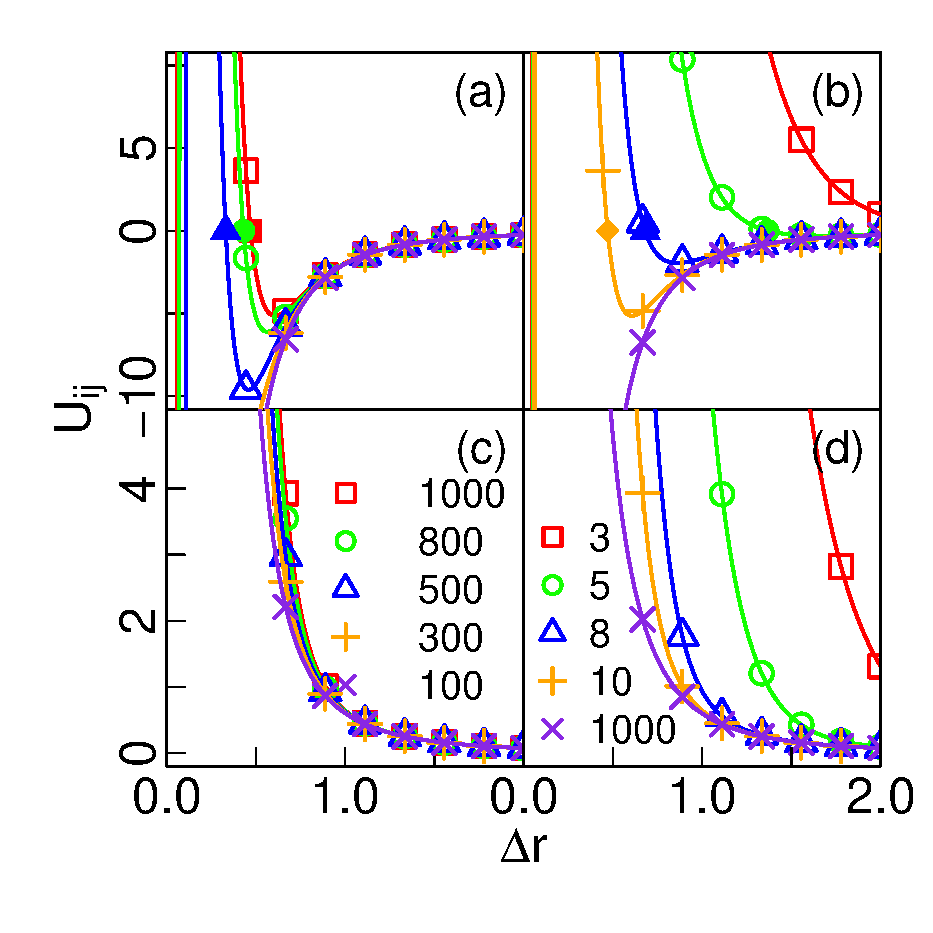
\includegraphics[width=0.9\columnwidth]{Images/particle_interaction_potential}
\caption{Total energy of the pairwise interaction as function of the interparticle distance when both dipoles are aligned (top) or one is perpendicular (bottom) to the $z$ axis. For the plots a) and c) we fix the interaction range $k = 10$ while changing $A$, and for b) and d) we fix $A = 1000$ while changing $k$.}
\label{fig:interaction_energy}
\end{figure}
When two dipole moments are perpendicular to each other, the interaction is purely repulsive for any given $A$ and $k$. However, as we can see from Figs.~\ref{fig:interaction_energy}(a)~and~(b), for co-aligned configurations for significantly low values of $A$ and high values of $k$, the interaction is purely attractive. In this work, to reduce the number of free parameters we fix $A = 1000 \mu$ and $k = 10$.
